\ifdefined\ishandout
\documentclass[handout]{beamer}
\else
\documentclass{beamer}
\fi

\usepackage[frenchb]{babel}
\usepackage[T1]{fontenc}
\usepackage[latin1]{inputenc}
\usepackage{hyperref}
\usepackage{multirow}
\usepackage{listings}
\usepackage{fancyvrb}
\usepackage{tikz}
\usepackage{framed}
\usepackage{algorithm}
\usepackage{algorithmic}
\usepackage{xcolor}
\usepackage{color, colortbl}
\usepackage{handoutWithNotes}
\usetikzlibrary{shapes.geometric}
\usetikzlibrary{shapes.arrows, chains}
\usetikzlibrary{arrows,calc}
\usepackage{array}
\usetheme{Boadilla}

\ifdefined\ishandout
\pgfpagesuselayout{3 on 1 with notes}[a4paper,border shrink=5mm]
\usecolortheme{dove}
\else
\usecolortheme{dolphin}
\fi


\lstnewenvironment{codeC}
{ \lstset{language=C,
    otherkeywords={printf,scanf}}
}
{}

\ifdefined\ishandout
\definecolor{mygreen}{rgb}{0,0,0}
\definecolor{mymauve}{rgb}{0,0,0}
\definecolor{myblue}{rgb}{0,0,0}
\else
\definecolor{mygreen}{rgb}{0,0.6,0}
\definecolor{mymauve}{rgb}{0.58,0,0.82}
\definecolor{myblue}{rgb}{0,0,1}

\fi

\definecolor{mygray}{rgb}{0.5,0.5,0.5}


\lstset{language=C,
% breakatwhitespace=false,         % sets if automatic breaks should only happen at whitespace
%  breaklines=true,                 % sets automatic line breaking
%  captionpos=b,                
commentstyle=\itshape\color{mymauve},
keywordstyle=\bfseries\color{myblue},
%numbers=left,                    % where to put the line-numbers; possible values are (none, left, right)
%  numbersep=8pt,                   % how far the line-numbers are from the code
%  numberstyle=\tiny\color{mygray}, % the style that is used for the line-numbers
  rulecolor=\color{black},         % if not set, the frame-color may be changed on line-breaks within not-black text (e.g. comments (green here))
%  showspaces=false,                % show spaces everywhere adding particular underscores; it overrides 'showstringspaces'
  showstringspaces=false,          % underline spaces within strings only
%  showtabs=false,                  % show tabs within strings adding particular underscores
%  stepnumber=2,                    % the step between two line-numbers. If it's 1, each line will be numbered
  stringstyle=\color{mygreen},     % string literal style
%  tabsize=2 
}

\newcommand{\red}{\textcolor{red}}
%\newcommand \emph
%Default size : 12.8 cm * 9.6 cm

\ifdefined\ishandout
\newenvironment<>{codeblock}[1]{%begin
  \setbeamercolor{block title}{fg=black,bg=lightgray!80}%
  \begin{block}{#1}}
  % \begin{codeC}}
  %  {\end{codeC}
{  
\end{block}}

\newenvironment<>{termblock}[1]{
    \setbeamercolor{block title}{fg=black,bg=lightgray!90}%
    \begin{block}{#1}
}
%     \begin{Verbatim}}
{%\end{Verbatim}
\end{block}
}

\definecolor{bluegreen}{RGB}{0,0,0}
%\definecolor{bluegreen}{rgb}{0,0.6,0.8}
\else

\newenvironment<>{codeblock}[1]{%begin
  \setbeamercolor{block title}{fg=darkgray,bg=yellow}%
  \begin{block}{#1}}
  % \begin{codeC}}
  %  {\end{codeC}
{  
\end{block}}

\newenvironment<>{termblock}[1]{
    \setbeamercolor{block title}{fg=white,bg=lightgray}%
    \begin{block}{#1}}
%     \begin{Verbatim}}
{%\end{Verbatim}
\end{block}
}

\definecolor{bluegreen}{RGB}{0,149,182}
%\definecolor{bluegreen}{rgb}{0,0.6,0.8}
\fi

%\newcommand{\output}[1]{
\setbeamertemplate{navigation symbols}{}
\newcommand{\bvrb}{\Verb[commandchars=���,formatcom=\color{bluegreen}]}
\newcommand{\footvrb}{\footnotesize\Verb}


%%% Param�tres du cours (� r�gler)
%Num�ro du cours
\newcommand{\nb}{4}

\title[Cours n�\nb]{Cours n�\nb - Les Fonctions}
\author[]{julien.brajard@upmc.fr}
\institute[Polytech' UPMC]{Polytech' UPMC}
\date{19 Octobre 2015}
\begin{document}
%%%%%%%%%%%%%%%%%%%%% SLIDES DE TITRE
\begin{frame}
\titlepage
\centering{
\url{http://australe.upmc.fr} (onglet EPU-C5-IGE Info Gen)}
\end{frame}
%%%%%%%%%%%%%%%%%%%%%
\begin{frame}
\frametitle{Plan du cours n�\nb}
\tableofcontents[hideallsubsections]
\end{frame}

%%%%



%%%%%% SECTION 12
% !TEX encoding = IsoLatin9

%%%�%%%%%%%%%%%%%%%%%% SECTION 1
\section{Les fonctions}
\begin{frame}
  \begin{columns}
    \column{4.8cm}
    \tableofcontents[currentsection,hideothersubsections]
    \column{7cm}
    
  \end{columns}
  
\end{frame}


\begin{frame}
\frametitle{Introduction}
\begin{itemize}
\setlength\itemsep{1em}
\item La r�solution d'un probl�me informatique
peut conduire � la r�solution de plusieurs probl�mes
plus �l�mentaires.
\begin{itemize}
\item Exemple des traitements des tableaux
\end{itemize}
\item Id�e :
\begin{itemize}
\item Identifier ces traitements �l�mentaires 
pour la r�solution du probl�me initial.
\item Construire des petits programmes pour chacun
des traitements �l�mentaires (et les \red{tester}).
\item Ecrire un programme final simple qui utilise
les programmes �l�mentaires comme des briques de base.
\end{itemize}
\end{itemize}
\end{frame}

\begin{frame}
\frametitle{Solution : les fonctions}
\begin{block}{}
Le langage C permet ce d�coupage.
C'est la programmation modulaire.
\end{block}
\begin{itemize}
\item Permet de d�couper un traitement en autant
de traitements �l�mentaires qu'on le souhaite.
\item Permet d'appeler des modules existants (biblioth�que).
\item Permet de d�finir ses modules et de construire ses propres
biblioth�ques.
\item Permet de d�couper un gros logiciel pour faciliter sa mise au point.
\item Evite des copier-coller de code et am�liore sa visibilit�.
\item Permet le travail collaboratif.
\end{itemize}
\end{frame}

\begin{frame}[fragile]
\frametitle{Qu'est-ce qu'une fonction ?}
\begin{alertblock}{}
Une fonction est sous-programme pouvant �tre
appel� dans un programme et qui effectue une 
suite d'op�rations.

Les op�rations effectu�es peuvent d�pendre
de 1 ou plusieurs entr�es et la fonction peut 
renvoyer \red{au plus} une seule sortie (en langage C).
\end{alertblock}
\vspace{1cm}
\begin{figure}
\centering
\begin{tikzpicture} [
       auto,
       function/.style={diamond, draw=blue,thick,fill=blue!20,
               text width = 2cm, text badly centered, rounded corners,
               aspect=2},
       texte/.style={text width = 2cm,text badly centered},
        line/.style     = { draw, thick, ->, shorten >=2pt },
       node distance=4cm,
       ]
       \node (input) [texte]{Entiers, tableaux, r�els, ...};
       \node (fonc) [function, right of = input] {La fonction};
       \node (output) [texte, right of = fonc] {\textbf{Un} entier ou \textbf{Un} r�el, ou ...};
        \begin{scope}[every path/.style=line]
        \path (input) -- (fonc) ;
        \path (fonc) -- (output); 
\end{scope}
\end{tikzpicture}
\end{figure}
\end{frame}

\begin{frame}[fragile]
\frametitle<1>{Exemple : la fonction max}
\frametitle<2>{Terminologie}

\visible<2>{\red{\textbf{D�claration : }}}
\begin{figure}
\centering
\begin{tikzpicture} [
       auto,
       function/.style={diamond, draw=blue,thick,fill=blue!20,
               text width = 2cm, text badly centered, rounded corners,
               aspect=2},
       texte/.style={text width = 2cm,text badly centered},
        line/.style     = { draw, thick, ->, shorten >=2pt },
       node distance=4cm,
       ]
       \node (input) [texte]{Un entier \textbf{a}, Un entier \textbf{b}};
       \node (fonc) [function, right of = input] {max};
       \node (output) [texte, right of = fonc] {\textbf{Un entier} (maximum entre a et b)};
        \begin{scope}[every path/.style=line]
        \path (input) -- (fonc) ;
        \path (fonc) -- (output); 
\end{scope}
\end{tikzpicture}
\end{figure}

\visible<2>{\red{\textbf{Appel : }}}
\begin{figure}
\centering
\begin{tikzpicture} [
       auto,
       function/.style={diamond, draw=blue,thick,fill=blue!20,
               text width = 2cm, text badly centered, rounded corners,
               aspect=2},
       texte/.style={text width = 2cm,text badly centered},
        line/.style     = { draw, thick, ->, shorten >=2pt },
       node distance=4cm,
       ]
       \node (input) [texte]{2\\3};
       \node (fonc) [function, right of = input] {max};
       \node (output) [texte, right of = fonc] {3};
        \begin{scope}[every path/.style=line]
        \path (input) -- (fonc) ;
        \path (fonc) -- (output); 
\end{scope}
\end{tikzpicture}
\end{figure}

\visible<2>{\red{\textbf{D�finition : }}}
\begin{figure}
\centering
\begin{tikzpicture} [
       auto,
       function/.style={diamond, draw=blue,thick,fill=blue!20,
               text width = 2cm, text badly centered, rounded corners,
               aspect=2},
       texte/.style={text width = 2cm,text badly centered},
        line/.style     = { draw, thick, ->, shorten >=2pt },
       node distance=4cm,
       ]
       \node (input) [texte]{Un entier \textbf{a}, Un entier \textbf{b}};
       \node (fonc) [function, right of = input, text width = 3cm, inner sep = 0pt] {{\footnotesize si a<b, renvoyer b\\sinon renvoyer a}};
       \node (output) [texte, right of = fonc] { \textbf{Un entier} (maximum entre a et b)} ;
        \begin{scope}[every path/.style=line]
        \path (input) -- (fonc) ;
        \path (fonc) -- (output); 
\end{scope}
\end{tikzpicture}
\end{figure}
\end{frame}

\begin{frame}[fragile]
\frametitle{En langage C}
\begin{itemize}
\setlength\itemsep{1em}
\item D�claration (le \red{prototype} de la fonction) :\\
\bvrb|�textit�type_retour nom_fonction�(�textit�arguments�);|\\
\item Appel :\\
\bvrb|�textit�nom_fonction�(�textit�liste_valeurs�);|\\
\item D�finition :\\
\bvrb|�textit�type_retour nom_fonction�(�textit�arguments�);|\\
\bvrb|{|\\
\bvrb|�textit�d�claration de variables locales�|\\
\bvrb|�textit�bloc d'instructions�|\\
\bvrb|return �textit�valeur_retour�;|\\
\bvrb|}|
\end{itemize}
\end{frame}

\begin{frame}[fragile]
\frametitle{La fonction \Verb|max|}

\begin{itemize}
\setlength\itemsep{1em}
\item D�claration :\\
\begin{codeblock}{}
\vspace{-.3cm}
\lstset{escapeinside={��}}
\lstset{basicstyle=\scriptsize}
\begin{codeC}
int max (int a, int b);
\end{codeC}
\vspace{-.3cm}
\end{codeblock}

\item Appel :\\
\begin{codeblock}{}
\vspace{-.3cm}
\lstset{escapeinside={��}}
\lstset{basicstyle=\scriptsize}
\begin{codeC}
int maxi ;
int n ;
scanf("%d",&n);
maxi = max(n,3); //Appel de la fonction max
\end{codeC}
\vspace{-.3cm}
\end{codeblock}

\item D�finition :\\
\begin{codeblock}{}
\vspace{-.3cm}
\lstset{escapeinside={��}}
\lstset{basicstyle=\scriptsize}
\begin{codeC}
int max (int a, int b)
{
  if (a<b) return(b) ;
  else return(a) ;
}
\end{codeC}
\vspace{-.3cm}
\end{codeblock}

\end{itemize}
\end{frame}

\begin{frame}[fragile]
\frametitle{Quelque r�gles}
\begin{itemize}
\setlength\itemsep{1em}
\item Une fonction peut �tre d�finie n'importe o� dans le programme ;
\item Une fonction doit �tre d�clar�e avant d'�tre d�clar�e avant d'�tre appel�e pour
la premi�re fois ;
\item Une fonction peut �tre appel�e dans le \bvrb|main| ou dans
une autre fonction ;
\item On ne peut \red{pas} d�finir une fonction dans une autre fonction ;
\item Une fonction peut prendre autant d'argument que l'on souhaite
en entr�e mais ne retour qu'un plus un �l�ment ;
\item Les r�gles sur les noms de fonctions sont les m�mes que
sur les noms de variables.
\end{itemize}
\end{frame}

\begin{frame}[fragile]
\frametitle{Tol�rance}
\begin{block}{}
Si l'on d�finit une fonction avant de l'appeler, on peut �ventuellement
se passer de la d�clarer.
\end{block}
\begin{columns}
\column{.4\textwidth}
\begin{codeblock}{}
\vspace{-.3cm}
\lstset{escapeinside={��}}
\lstset{basicstyle=\scriptsize}
\begin{codeC}
//D�claration-D�finition
int max (int a, int b) {
  if (a<b) return (b) ;
  else return (a) ;
}

//Fonction principale
int main() {
  int maxi, n ;
  scanf("%d",&n);
  maxi = max (n,3);
  printf("%d\n",maxi);
}
\end{codeC}
\vspace{-.3cm}
\end{codeblock}

\column{.15\textwidth}
{\centering {\footnotesize Equivalent
$$\Leftrightarrow$$}}

\column{.4\textwidth}
\begin{codeblock}{}
\vspace{-.3cm}
\lstset{escapeinside={��}}
\lstset{basicstyle=\scriptsize}
\begin{codeC}
//D�claration
int max (int a, int b) ;

//Fonction principale
int main() {
  int maxi, n ;
  scanf("%d",&n);
  maxi = max (n,3);
  printf("%d\n",maxi);
}

//D�finition
int max (int a, int b) {
  if (a<b) return (b) ;
  else return (a) ;
}

\end{codeC}
\vspace{-.3cm}
\end{codeblock}


\end{columns}
\end{frame}

\begin{frame}[fragile]
\frametitle{Fonction appel�e / Fonction appelante}
\begin{columns}
\column{0.45\textwidth}
\begin{codeblock}{}
\vspace{-.3cm}
\lstset{escapeinside={��}}
\lstset{basicstyle=\scriptsize}
\begin{codeC}
//D�claration des fonctions
int f(int a);
int g(int b);

//Fonction principale
int main() {
  int z = 2 ;
  z = g(z) + f(z) ;
  printf("%d\n",z);
 }

//D�finition des fonctions
int f (int a) {
  return (a+2) ;
}

int g (int b) {
  return ( 2*f(b) ) ;
}
\end{codeC}
\vspace{-.3cm}
\end{codeblock}
\column{0.5\textwidth}
\begin{block}{}
Une fonction peut �tre appel�e de n'importe
quelle fonction y compris dans le
\bvrb|main|
\end{block}

\begin{itemize}
\item Fonctions appelantes :
\begin{itemize}
\item \Verb|main| appelle \Verb|g| et \Verb|f|
\item \Verb|g| appelle \Verb|f|
\end{itemize}
\item Fonctions appel�es :
\begin{itemize}
\item \Verb|f| est appel�e par \Verb|main| et \Verb|g|
\item \Verb|g| est appel�e par \Verb|main|
\end{itemize}
\end{itemize}
\end{columns}
\end{frame}
\end{document} 

%%%%%%%%%%%%%%%%%%%%% SECTION 1
\section{Les algorithmes}\label{section:1}
\begin{frame}
\begin{columns}
        \column{4.8cm}
            \tableofcontents[currentsection]
        \column{7cm}
        \centering{
            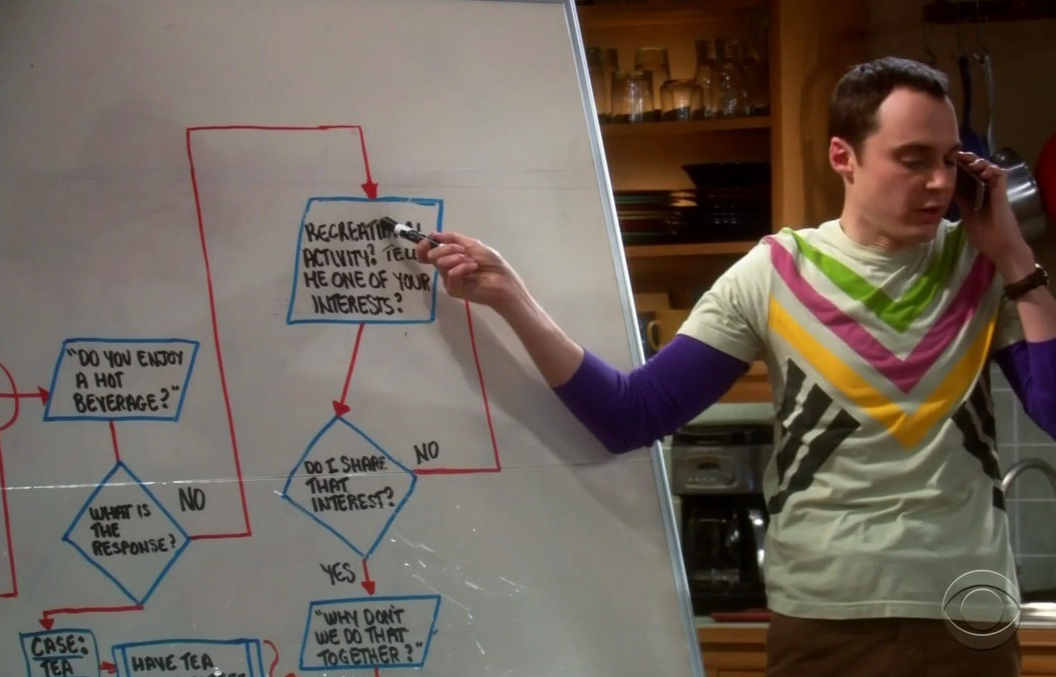
\includegraphics[width=7cm]{fig/Algorithm-sheldon.png}
            
                 \textit{ I believe I've isolateblblblblblblsblbslbslbsl
            sblbslblsblsblblsblbs
            lbslblbslsb d the algorithm for making friends.}
     
            
            \small{
            \hfill Sheldon Cooper, 
            
            \hfill in \textit{The Big Band Theory}, Season 2, Episode 13
            }
}

    \end{columns}

\end{frame}


%%%%%%%%%%%%%%%%%%%%%
\subsection{Introduction}
    \begin{frame}
    \frametitle{Pourquoi faire appel � des algorithmes ?}
    Pour automatiser des t�ches
    
    Exemples :
    \begin{itemize}
    \item M�tier � tisser\\
    \item M�thode de calcul � la main d'une division\\
    \item Recette de cuisine\\
    \item ...\\
    \end{itemize}
    \end{frame}
 
 %%%%%%%%%%%%%%%%%
 
    \begin{frame}
    \frametitle{Qu'est-ce qu'un algorithme ?}
    \begin{block}{D�finition}
    Un algorithme est un ensemble 
    ordonn� d'instructions simples
permettant de r�soudre un probl�me.
    \end{block}
    \end{frame}
    
 %%%%%%%%%%%%%%%%%%
 \subsection{Construction d'un algorithme}
%%%%%%%%%%%%%%%%%%%    
\section{La machine de Turing}
%%%%%%%%%%%%%%%%%%%%
 
  
\begin{frame}[fragile]
\frametitle{Un peu d'histoire...}
\begin{codeblock}{Test}
\begin{codeC}
for (int i = 0 ; i < n ; i ++) {
    //a comment
    printf("%d",i);
    }
\end{codeC}
\end{codeblock}

\begin{termblock}{test 2}
\lstset{escapeinside={��}}
\begin{lstlisting}
�\textbf{>>}�./a.out
�\color{darkgray}{\texttt{  Hello World}}�
\end{lstlisting}
\end{termblock}

 \begin{block}{Bloc standard}
blablabla
\end{block}
\end{frame}


\begin{frame}[fragile]
\frametitle{essai}
\begin{columns}
\column{6cm}
\begin{block}

\begin{figure}
\begin{tikzpicture} [
    auto,
    decision/.style = { diamond, draw=blue, thick, fill=blue!20,
                        text width=5em, text badly centered,
                        inner sep=1pt, rounded corners },
    block/.style    = { rectangle, draw=blue, thick, 
                        fill=blue!20, text width=10em, text centered,
                        rounded corners, minimum height=2em },
    line/.style     = { draw, thick, ->, shorten >=2pt },
  ]
   \matrix [column sep=-10mm, row sep=10mm] {
                    & \node [text centered] (x) {$\mathbf{X}$};            & \\
                    & \node (null1) {};                                    & \\
                    & \node [block] (doa) {\textsf{DoAE}($\mathbf{X}$)};   & \\
  	               \node(null3){}; & \node [decision] (uiddes)
                        {\textsf{UID}($\hat{\mathbf{X}}$)};
                                  & \node[text centered](tra){$\mathbf{i}$}; \\
                  & \node [block] (track) {\textsf{DoAT}($\mathbf{x}$)}; & \\
                    & \node [block] (pesos)
                        {\textsf{BF}(DoA$_{\mathrm{T}}$,DoAs)};            & \\
                    & \node [block] (filtrado)
                        {\textsf{SF}($\mathbf{w}$,$\mathbf{x}$)};          & \\
                    & \node [text centered] (xf) {$\hat{x}(t)$ };          & \\
  };
  % connect all nodes defined above
 \begin{scope} [every path/.style=line]
    \path (x)        --    (doa);
    \path (doa)      --    node [near start] {DoAs} (uiddes);
    \path (tra)      --    (uiddes);
    \path (uiddes)   --++  (-3,0) node [near start] {no} |- (null1);
    \path (uiddes)   --    node [near start] {DoA} (track);
    \path (track)    --    node [near start] {DoA$_{\mathrm{T}}$} (pesos);
    \path (pesos)    --    node [near start] {\textbf{w}} (filtrado);
    \path (filtrado) --    (xf);
  
  \end{scope}
\end{tikzpicture}
\end{figure}
\end{block}
\column{3cm}
\begin{block}{bulbul}
\end{block}
\end{columns}
\end{frame}

\end{document}
